\documentclass[10pt]{article}
\usepackage{tmlr}
% \usepackage[preprint]{tmlr}   % de-anonymised preprint version
%%%%% NEW MATH DEFINITIONS %%%%%

\usepackage{amsmath,amsfonts,bm}

% Mark sections of captions for referring to divisions of figures
\newcommand{\figleft}{{\em (Left)}}
\newcommand{\figcenter}{{\em (Center)}}
\newcommand{\figright}{{\em (Right)}}
\newcommand{\figtop}{{\em (Top)}}
\newcommand{\figbottom}{{\em (Bottom)}}
\newcommand{\captiona}{{\em (a)}}
\newcommand{\captionb}{{\em (b)}}
\newcommand{\captionc}{{\em (c)}}
\newcommand{\captiond}{{\em (d)}}

% Highlight a newly defined term
\newcommand{\newterm}[1]{{\bf #1}}


% Figure reference, lower-case.
\def\figref#1{figure~\ref{#1}}
% Figure reference, capital. For start of sentence
\def\Figref#1{Figure~\ref{#1}}
\def\twofigref#1#2{figures \ref{#1} and \ref{#2}}
\def\quadfigref#1#2#3#4{figures \ref{#1}, \ref{#2}, \ref{#3} and \ref{#4}}
% Section reference, lower-case.
\def\secref#1{section~\ref{#1}}
% Section reference, capital.
\def\Secref#1{Section~\ref{#1}}
% Reference to two sections.
\def\twosecrefs#1#2{sections \ref{#1} and \ref{#2}}
% Reference to three sections.
\def\secrefs#1#2#3{sections \ref{#1}, \ref{#2} and \ref{#3}}
% Reference to an equation, lower-case.
\def\eqref#1{equation~\ref{#1}}
% Reference to an equation, upper case
\def\Eqref#1{Equation~\ref{#1}}
% A raw reference to an equation---avoid using if possible
\def\plaineqref#1{\ref{#1}}
% Reference to a chapter, lower-case.
\def\chapref#1{chapter~\ref{#1}}
% Reference to an equation, upper case.
\def\Chapref#1{Chapter~\ref{#1}}
% Reference to a range of chapters
\def\rangechapref#1#2{chapters\ref{#1}--\ref{#2}}
% Reference to an algorithm, lower-case.
\def\algref#1{algorithm~\ref{#1}}
% Reference to an algorithm, upper case.
\def\Algref#1{Algorithm~\ref{#1}}
\def\twoalgref#1#2{algorithms \ref{#1} and \ref{#2}}
\def\Twoalgref#1#2{Algorithms \ref{#1} and \ref{#2}}
% Reference to a part, lower case
\def\partref#1{part~\ref{#1}}
% Reference to a part, upper case
\def\Partref#1{Part~\ref{#1}}
\def\twopartref#1#2{parts \ref{#1} and \ref{#2}}

\def\ceil#1{\lceil #1 \rceil}
\def\floor#1{\lfloor #1 \rfloor}
\def\1{\bm{1}}
\newcommand{\train}{\mathcal{D}}
\newcommand{\valid}{\mathcal{D_{\mathrm{valid}}}}
\newcommand{\test}{\mathcal{D_{\mathrm{test}}}}

\def\eps{{\epsilon}}


% Random variables
\def\reta{{\textnormal{$\eta$}}}
\def\ra{{\textnormal{a}}}
\def\rb{{\textnormal{b}}}
\def\rc{{\textnormal{c}}}
\def\rd{{\textnormal{d}}}
\def\re{{\textnormal{e}}}
\def\rf{{\textnormal{f}}}
\def\rg{{\textnormal{g}}}
\def\rh{{\textnormal{h}}}
\def\ri{{\textnormal{i}}}
\def\rj{{\textnormal{j}}}
\def\rk{{\textnormal{k}}}
\def\rl{{\textnormal{l}}}
% rm is already a command, just don't name any random variables m
\def\rn{{\textnormal{n}}}
\def\ro{{\textnormal{o}}}
\def\rp{{\textnormal{p}}}
\def\rq{{\textnormal{q}}}
\def\rr{{\textnormal{r}}}
\def\rs{{\textnormal{s}}}
\def\rt{{\textnormal{t}}}
\def\ru{{\textnormal{u}}}
\def\rv{{\textnormal{v}}}
\def\rw{{\textnormal{w}}}
\def\rx{{\textnormal{x}}}
\def\ry{{\textnormal{y}}}
\def\rz{{\textnormal{z}}}

% Random vectors
\def\rvepsilon{{\mathbf{\epsilon}}}
\def\rvtheta{{\mathbf{\theta}}}
\def\rva{{\mathbf{a}}}
\def\rvb{{\mathbf{b}}}
\def\rvc{{\mathbf{c}}}
\def\rvd{{\mathbf{d}}}
\def\rve{{\mathbf{e}}}
\def\rvf{{\mathbf{f}}}
\def\rvg{{\mathbf{g}}}
\def\rvh{{\mathbf{h}}}
\def\rvu{{\mathbf{i}}}
\def\rvj{{\mathbf{j}}}
\def\rvk{{\mathbf{k}}}
\def\rvl{{\mathbf{l}}}
\def\rvm{{\mathbf{m}}}
\def\rvn{{\mathbf{n}}}
\def\rvo{{\mathbf{o}}}
\def\rvp{{\mathbf{p}}}
\def\rvq{{\mathbf{q}}}
\def\rvr{{\mathbf{r}}}
\def\rvs{{\mathbf{s}}}
\def\rvt{{\mathbf{t}}}
\def\rvu{{\mathbf{u}}}
\def\rvv{{\mathbf{v}}}
\def\rvw{{\mathbf{w}}}
\def\rvx{{\mathbf{x}}}
\def\rvy{{\mathbf{y}}}
\def\rvz{{\mathbf{z}}}

% Elements of random vectors
\def\erva{{\textnormal{a}}}
\def\ervb{{\textnormal{b}}}
\def\ervc{{\textnormal{c}}}
\def\ervd{{\textnormal{d}}}
\def\erve{{\textnormal{e}}}
\def\ervf{{\textnormal{f}}}
\def\ervg{{\textnormal{g}}}
\def\ervh{{\textnormal{h}}}
\def\ervi{{\textnormal{i}}}
\def\ervj{{\textnormal{j}}}
\def\ervk{{\textnormal{k}}}
\def\ervl{{\textnormal{l}}}
\def\ervm{{\textnormal{m}}}
\def\ervn{{\textnormal{n}}}
\def\ervo{{\textnormal{o}}}
\def\ervp{{\textnormal{p}}}
\def\ervq{{\textnormal{q}}}
\def\ervr{{\textnormal{r}}}
\def\ervs{{\textnormal{s}}}
\def\ervt{{\textnormal{t}}}
\def\ervu{{\textnormal{u}}}
\def\ervv{{\textnormal{v}}}
\def\ervw{{\textnormal{w}}}
\def\ervx{{\textnormal{x}}}
\def\ervy{{\textnormal{y}}}
\def\ervz{{\textnormal{z}}}

% Random matrices
\def\rmA{{\mathbf{A}}}
\def\rmB{{\mathbf{B}}}
\def\rmC{{\mathbf{C}}}
\def\rmD{{\mathbf{D}}}
\def\rmE{{\mathbf{E}}}
\def\rmF{{\mathbf{F}}}
\def\rmG{{\mathbf{G}}}
\def\rmH{{\mathbf{H}}}
\def\rmI{{\mathbf{I}}}
\def\rmJ{{\mathbf{J}}}
\def\rmK{{\mathbf{K}}}
\def\rmL{{\mathbf{L}}}
\def\rmM{{\mathbf{M}}}
\def\rmN{{\mathbf{N}}}
\def\rmO{{\mathbf{O}}}
\def\rmP{{\mathbf{P}}}
\def\rmQ{{\mathbf{Q}}}
\def\rmR{{\mathbf{R}}}
\def\rmS{{\mathbf{S}}}
\def\rmT{{\mathbf{T}}}
\def\rmU{{\mathbf{U}}}
\def\rmV{{\mathbf{V}}}
\def\rmW{{\mathbf{W}}}
\def\rmX{{\mathbf{X}}}
\def\rmY{{\mathbf{Y}}}
\def\rmZ{{\mathbf{Z}}}

% Elements of random matrices
\def\ermA{{\textnormal{A}}}
\def\ermB{{\textnormal{B}}}
\def\ermC{{\textnormal{C}}}
\def\ermD{{\textnormal{D}}}
\def\ermE{{\textnormal{E}}}
\def\ermF{{\textnormal{F}}}
\def\ermG{{\textnormal{G}}}
\def\ermH{{\textnormal{H}}}
\def\ermI{{\textnormal{I}}}
\def\ermJ{{\textnormal{J}}}
\def\ermK{{\textnormal{K}}}
\def\ermL{{\textnormal{L}}}
\def\ermM{{\textnormal{M}}}
\def\ermN{{\textnormal{N}}}
\def\ermO{{\textnormal{O}}}
\def\ermP{{\textnormal{P}}}
\def\ermQ{{\textnormal{Q}}}
\def\ermR{{\textnormal{R}}}
\def\ermS{{\textnormal{S}}}
\def\ermT{{\textnormal{T}}}
\def\ermU{{\textnormal{U}}}
\def\ermV{{\textnormal{V}}}
\def\ermW{{\textnormal{W}}}
\def\ermX{{\textnormal{X}}}
\def\ermY{{\textnormal{Y}}}
\def\ermZ{{\textnormal{Z}}}

% Vectors
\def\vzero{{\bm{0}}}
\def\vone{{\bm{1}}}
\def\vmu{{\bm{\mu}}}
\def\vtheta{{\bm{\theta}}}
\def\va{{\bm{a}}}
\def\vb{{\bm{b}}}
\def\vc{{\bm{c}}}
\def\vd{{\bm{d}}}
\def\ve{{\bm{e}}}
\def\vf{{\bm{f}}}
\def\vg{{\bm{g}}}
\def\vh{{\bm{h}}}
\def\vi{{\bm{i}}}
\def\vj{{\bm{j}}}
\def\vk{{\bm{k}}}
\def\vl{{\bm{l}}}
\def\vm{{\bm{m}}}
\def\vn{{\bm{n}}}
\def\vo{{\bm{o}}}
\def\vp{{\bm{p}}}
\def\vq{{\bm{q}}}
\def\vr{{\bm{r}}}
\def\vs{{\bm{s}}}
\def\vt{{\bm{t}}}
\def\vu{{\bm{u}}}
\def\vv{{\bm{v}}}
\def\vw{{\bm{w}}}
\def\vx{{\bm{x}}}
\def\vy{{\bm{y}}}
\def\vz{{\bm{z}}}

% Elements of vectors
\def\evalpha{{\alpha}}
\def\evbeta{{\beta}}
\def\evepsilon{{\epsilon}}
\def\evlambda{{\lambda}}
\def\evomega{{\omega}}
\def\evmu{{\mu}}
\def\evpsi{{\psi}}
\def\evsigma{{\sigma}}
\def\evtheta{{\theta}}
\def\eva{{a}}
\def\evb{{b}}
\def\evc{{c}}
\def\evd{{d}}
\def\eve{{e}}
\def\evf{{f}}
\def\evg{{g}}
\def\evh{{h}}
\def\evi{{i}}
\def\evj{{j}}
\def\evk{{k}}
\def\evl{{l}}
\def\evm{{m}}
\def\evn{{n}}
\def\evo{{o}}
\def\evp{{p}}
\def\evq{{q}}
\def\evr{{r}}
\def\evs{{s}}
\def\evt{{t}}
\def\evu{{u}}
\def\evv{{v}}
\def\evw{{w}}
\def\evx{{x}}
\def\evy{{y}}
\def\evz{{z}}

% Matrix
\def\mA{{\bm{A}}}
\def\mB{{\bm{B}}}
\def\mC{{\bm{C}}}
\def\mD{{\bm{D}}}
\def\mE{{\bm{E}}}
\def\mF{{\bm{F}}}
\def\mG{{\bm{G}}}
\def\mH{{\bm{H}}}
\def\mI{{\bm{I}}}
\def\mJ{{\bm{J}}}
\def\mK{{\bm{K}}}
\def\mL{{\bm{L}}}
\def\mM{{\bm{M}}}
\def\mN{{\bm{N}}}
\def\mO{{\bm{O}}}
\def\mP{{\bm{P}}}
\def\mQ{{\bm{Q}}}
\def\mR{{\bm{R}}}
\def\mS{{\bm{S}}}
\def\mT{{\bm{T}}}
\def\mU{{\bm{U}}}
\def\mV{{\bm{V}}}
\def\mW{{\bm{W}}}
\def\mX{{\bm{X}}}
\def\mY{{\bm{Y}}}
\def\mZ{{\bm{Z}}}
\def\mBeta{{\bm{\beta}}}
\def\mPhi{{\bm{\Phi}}}
\def\mLambda{{\bm{\Lambda}}}
\def\mSigma{{\bm{\Sigma}}}

% Tensor
\DeclareMathAlphabet{\mathsfit}{\encodingdefault}{\sfdefault}{m}{sl}
\SetMathAlphabet{\mathsfit}{bold}{\encodingdefault}{\sfdefault}{bx}{n}
\newcommand{\tens}[1]{\bm{\mathsfit{#1}}}
\def\tA{{\tens{A}}}
\def\tB{{\tens{B}}}
\def\tC{{\tens{C}}}
\def\tD{{\tens{D}}}
\def\tE{{\tens{E}}}
\def\tF{{\tens{F}}}
\def\tG{{\tens{G}}}
\def\tH{{\tens{H}}}
\def\tI{{\tens{I}}}
\def\tJ{{\tens{J}}}
\def\tK{{\tens{K}}}
\def\tL{{\tens{L}}}
\def\tM{{\tens{M}}}
\def\tN{{\tens{N}}}
\def\tO{{\tens{O}}}
\def\tP{{\tens{P}}}
\def\tQ{{\tens{Q}}}
\def\tR{{\tens{R}}}
\def\tS{{\tens{S}}}
\def\tT{{\tens{T}}}
\def\tU{{\tens{U}}}
\def\tV{{\tens{V}}}
\def\tW{{\tens{W}}}
\def\tX{{\tens{X}}}
\def\tY{{\tens{Y}}}
\def\tZ{{\tens{Z}}}


% Graph
\def\gA{{\mathcal{A}}}
\def\gB{{\mathcal{B}}}
\def\gC{{\mathcal{C}}}
\def\gD{{\mathcal{D}}}
\def\gE{{\mathcal{E}}}
\def\gF{{\mathcal{F}}}
\def\gG{{\mathcal{G}}}
\def\gH{{\mathcal{H}}}
\def\gI{{\mathcal{I}}}
\def\gJ{{\mathcal{J}}}
\def\gK{{\mathcal{K}}}
\def\gL{{\mathcal{L}}}
\def\gM{{\mathcal{M}}}
\def\gN{{\mathcal{N}}}
\def\gO{{\mathcal{O}}}
\def\gP{{\mathcal{P}}}
\def\gQ{{\mathcal{Q}}}
\def\gR{{\mathcal{R}}}
\def\gS{{\mathcal{S}}}
\def\gT{{\mathcal{T}}}
\def\gU{{\mathcal{U}}}
\def\gV{{\mathcal{V}}}
\def\gW{{\mathcal{W}}}
\def\gX{{\mathcal{X}}}
\def\gY{{\mathcal{Y}}}
\def\gZ{{\mathcal{Z}}}

% Sets
\def\sA{{\mathbb{A}}}
\def\sB{{\mathbb{B}}}
\def\sC{{\mathbb{C}}}
\def\sD{{\mathbb{D}}}
% Don't use a set called E, because this would be the same as our symbol
% for expectation.
\def\sF{{\mathbb{F}}}
\def\sG{{\mathbb{G}}}
\def\sH{{\mathbb{H}}}
\def\sI{{\mathbb{I}}}
\def\sJ{{\mathbb{J}}}
\def\sK{{\mathbb{K}}}
\def\sL{{\mathbb{L}}}
\def\sM{{\mathbb{M}}}
\def\sN{{\mathbb{N}}}
\def\sO{{\mathbb{O}}}
\def\sP{{\mathbb{P}}}
\def\sQ{{\mathbb{Q}}}
\def\sR{{\mathbb{R}}}
\def\sS{{\mathbb{S}}}
\def\sT{{\mathbb{T}}}
\def\sU{{\mathbb{U}}}
\def\sV{{\mathbb{V}}}
\def\sW{{\mathbb{W}}}
\def\sX{{\mathbb{X}}}
\def\sY{{\mathbb{Y}}}
\def\sZ{{\mathbb{Z}}}

% Entries of a matrix
\def\emLambda{{\Lambda}}
\def\emA{{A}}
\def\emB{{B}}
\def\emC{{C}}
\def\emD{{D}}
\def\emE{{E}}
\def\emF{{F}}
\def\emG{{G}}
\def\emH{{H}}
\def\emI{{I}}
\def\emJ{{J}}
\def\emK{{K}}
\def\emL{{L}}
\def\emM{{M}}
\def\emN{{N}}
\def\emO{{O}}
\def\emP{{P}}
\def\emQ{{Q}}
\def\emR{{R}}
\def\emS{{S}}
\def\emT{{T}}
\def\emU{{U}}
\def\emV{{V}}
\def\emW{{W}}
\def\emX{{X}}
\def\emY{{Y}}
\def\emZ{{Z}}
\def\emSigma{{\Sigma}}

% entries of a tensor
% Same font as tensor, without \bm wrapper
\newcommand{\etens}[1]{\mathsfit{#1}}
\def\etLambda{{\etens{\Lambda}}}
\def\etA{{\etens{A}}}
\def\etB{{\etens{B}}}
\def\etC{{\etens{C}}}
\def\etD{{\etens{D}}}
\def\etE{{\etens{E}}}
\def\etF{{\etens{F}}}
\def\etG{{\etens{G}}}
\def\etH{{\etens{H}}}
\def\etI{{\etens{I}}}
\def\etJ{{\etens{J}}}
\def\etK{{\etens{K}}}
\def\etL{{\etens{L}}}
\def\etM{{\etens{M}}}
\def\etN{{\etens{N}}}
\def\etO{{\etens{O}}}
\def\etP{{\etens{P}}}
\def\etQ{{\etens{Q}}}
\def\etR{{\etens{R}}}
\def\etS{{\etens{S}}}
\def\etT{{\etens{T}}}
\def\etU{{\etens{U}}}
\def\etV{{\etens{V}}}
\def\etW{{\etens{W}}}
\def\etX{{\etens{X}}}
\def\etY{{\etens{Y}}}
\def\etZ{{\etens{Z}}}

% The true underlying data generating distribution
\newcommand{\pdata}{p_{\rm{data}}}
% The empirical distribution defined by the training set
\newcommand{\ptrain}{\hat{p}_{\rm{data}}}
\newcommand{\Ptrain}{\hat{P}_{\rm{data}}}
% The model distribution
\newcommand{\pmodel}{p_{\rm{model}}}
\newcommand{\Pmodel}{P_{\rm{model}}}
\newcommand{\ptildemodel}{\tilde{p}_{\rm{model}}}
% Stochastic autoencoder distributions
\newcommand{\pencode}{p_{\rm{encoder}}}
\newcommand{\pdecode}{p_{\rm{decoder}}}
\newcommand{\precons}{p_{\rm{reconstruct}}}

\newcommand{\laplace}{\mathrm{Laplace}} % Laplace distribution

\newcommand{\E}{\mathbb{E}}
\newcommand{\Ls}{\mathcal{L}}
\newcommand{\R}{\mathbb{R}}
\newcommand{\emp}{\tilde{p}}
\newcommand{\lr}{\alpha}
\newcommand{\reg}{\lambda}
\newcommand{\rect}{\mathrm{rectifier}}
\newcommand{\softmax}{\mathrm{softmax}}
\newcommand{\sigmoid}{\sigma}
\newcommand{\softplus}{\zeta}
\newcommand{\KL}{D_{\mathrm{KL}}}
\newcommand{\Var}{\mathrm{Var}}
\newcommand{\standarderror}{\mathrm{SE}}
\newcommand{\Cov}{\mathrm{Cov}}
% Wolfram Mathworld says $L^2$ is for function spaces and $\ell^2$ is for vectors
% But then they seem to use $L^2$ for vectors throughout the site, and so does
% wikipedia.
\newcommand{\normlzero}{L^0}
\newcommand{\normlone}{L^1}
\newcommand{\normltwo}{L^2}
\newcommand{\normlp}{L^p}
\newcommand{\normmax}{L^\infty}

\newcommand{\parents}{Pa} % See usage in notation.tex. Chosen to match Daphne's book.

\DeclareMathOperator*{\argmax}{arg\,max}
\DeclareMathOperator*{\argmin}{arg\,min}

\DeclareMathOperator{\sign}{sign}
\DeclareMathOperator{\Tr}{Tr}
\let\ab\allowbreak

\usepackage{hyperref}
\usepackage{url}
\usepackage{booktabs}
\usepackage{graphicx}
\usepackage{amsmath}
% generated by scripts/make_reconstruction_outputs.py - do not edit
\newcommand{\AccDeclineCommon}{0.016}
\newcommand{\AccDeclinePerYear}{0.024}
\newcommand{\AccDeclineSDCommon}{0.0005}
\newcommand{\AccDeclineSDPerYear}{0.0008}
\newcommand{\AccMaxDevCommon}{0.0090}
\newcommand{\AccMaxDevPerYear}{0.0024}
\newcommand{\AccMeanDevCommon}{0.0057}
\newcommand{\AccMeanDevPerYear}{0.0011}
\newcommand{\AccMeanDevTreesCCCommon}{0.0100}
\newcommand{\AccMeanDevTreesCCPerYear}{0.0018}
\newcommand{\AccMeanDevTreesCCommon}{0.0057}
\newcommand{\AccMeanDevTreesCPerYear}{0.0011}
\newcommand{\AccMeanDevTreesLCommon}{0.0026}
\newcommand{\AccMeanDevTreesLPerYear}{0.0037}
\newcommand{\DPMaxCommon}{0.158}
\newcommand{\DPMaxPerYear}{0.156}
\newcommand{\DPMinCommon}{0.152}
\newcommand{\DPMinPerYear}{0.152}
\newcommand{\EOMaxCommon}{0.160}
\newcommand{\EOMaxPerYear}{0.164}
\newcommand{\EOMinCommon}{0.156}
\newcommand{\EOMinPerYear}{0.154}
\newcommand{\ExpGradAccMaxDevCommon}{0.005}
\newcommand{\ExpGradAccMaxDevPerYear}{0.004}
\newcommand{\ExpGradDPMaxDevCommon}{0.011}
\newcommand{\ExpGradDPMaxDevPerYear}{0.014}
\newcommand{\LFRAccMaxDevCommon}{0.004}
\newcommand{\LFRAccMaxDevPerYear}{0.003}
\newcommand{\LFRDPMaxDevCommon}{0.006}
\newcommand{\LFRDPMaxDevPerYear}{0.004}
\newcommand{\LiteralAccGapMax}{0.15}
\newcommand{\LiteralAccGapMean}{0.12}
\newcommand{\LiteralAccGapMin}{0.10}
\newcommand{\PostAccMaxDevCommon}{0.022}
\newcommand{\PostAccMaxDevPerYear}{0.015}
\newcommand{\PostDPMaxDevCommon}{0.006}
\newcommand{\PostDPMaxDevPerYear}{0.013}
\newcommand{\PostEOAccGap}{0.038}
\newcommand{\PreprocContrastAcc}{0.0075}
\newcommand{\PreprocContrastShare}{29.5\%}
\newcommand{\PubAccDecline}{0.025}
\newcommand{\PubAccFirst}{0.823}
\newcommand{\PubAccLast}{0.798}
\newcommand{\PubDPMax}{0.165}
\newcommand{\PubDPMin}{0.163}
\newcommand{\PubEOMax}{0.209}
\newcommand{\PubEOMin}{0.175}
\newcommand{\ShareNotRecoveredCommon}{35.1\%}

\newcommand{\todo}[1]{\textcolor{red}{[TODO: #1]}}

\title{Does Fairness Stay Put? A Pre-Registered Re-Test of Temporal Fairness Stability on the American Community Survey, 2014--2024}

\author{\name Anonymous authors \email anonymous@example.com}

\def\month{MM}
\def\year{2026}
\def\openreview{\url{https://openreview.net/forum?id=XXXX}}

\begin{document}
\maketitle

\begin{abstract}
A widely cited result from the introduction of the folktables benchmarks holds that a classifier trained on 2014 US Census data keeps a nearly constant demographic-parity violation over 2015--2018, and that a classifier satisfying demographic parity in 2014 continues to satisfy it, even as its accuracy declines; fairness appeared more stable over time than across states.
We re-test this claim in a pre-registered extension built on a reconstructed pipeline. First, we reconstruct the original experiment on 2014--2018 data: among the variants we examined, the published accuracy curve is matched only with more boosting iterations than reported and with each survey year standardised separately; in our reconstruction, that preprocessing choice alone adds \PreprocContrastAcc{} to the 2014--2018 accuracy decline, \PreprocContrastShare{} of the published decline.
Second, with models fitted once and frozen before any later data were opened, we evaluate the claim at 2019 (race) and 2024 (sex) against tolerances fixed from 2014--2018 alone, for demographic parity and equality of opportunity, with and without survey weights.
Third, we compare temporal and cross-state change relative to geographic yardsticks and split temporal change into a composition part and a residual.
\todo{one sentence of results after Stage B.}
Code, frozen models and the documented feature harmonisation are released.
\end{abstract}

% ------------------------------------------------------------------
\section{Introduction}

Fairness interventions are usually certified once, on the data available at deployment, and then left in place while the population they act on changes.
Whether such certificates remain valid is an empirical question with direct consequences for monitoring and audit practice.
A prominent piece of evidence on this question for tabular decision-making comes from the paper that introduced the folktables datasets as a replacement for UCI Adult \citep{ding2021retiring}.
Using American Community Survey (ACS) data for 2014--2018, its authors found that a gradient-boosted classifier trained in 2014 lost some accuracy in later years while its demographic-parity violation stayed essentially constant, and that a classifier satisfying demographic parity in 2014 continued to satisfy it in 2015--2018.
Training and testing on different states, by contrast, gave unpredictable results, which led them to ask why fairness appears more stable over time than across space.

This claim is cited in both directions: as evidence that fairness properties persist under temporal shift, and as evidence that bias shifts over time \todo{citations from the citing-literature search}.
It also rests on a short window: five consecutive years, before the 2020 pandemic, the 2021--2023 inflation episode and several Census coding changes.
Seven more years of the same survey are now public.

We re-test the claim with three aims.
(i) \emph{Reconstruct} the original experiment and report precisely what reproduces it (Section~\ref{sec:reconstruction}).
(ii) \emph{Re-test} the claim on 2019 and 2021--2024 under a plan archived before any of those data were opened, with every model fitted and frozen beforehand, and with tolerances derived from 2014--2018 only (Sections~\ref{sec:design}--\ref{sec:results}). The models are built by our reconstructed, harmonised pipeline; the original fitted classifier is not available, so the re-test concerns the claim, not that classifier. The tests ask whether disparities at a later endpoint stay within the range seen in 2014--2018; they do not certify that a model is fair.
(iii) \emph{Explain} the pattern: compare temporal and geographic change relative to geographic yardsticks and split temporal change into a composition part and a residual, checking predictions from recent theory \citep{chen2022fairness,asiaee2026fairness}.

A point of logic shapes the design.
For a frozen classifier, the demographic-parity gap depends only on the distribution of the features within each group; the label never enters.
Changes in how income maps to the label, including inflation of a nominal income threshold, therefore cannot move it.
``Demographic parity stayed stable'' is thus a weak test on its own; the label-dependent quantities (accuracy, equality of opportunity) and the explanation of the temporal--geographic contrast carry the substantive weight, and we pre-registered them accordingly.

\paragraph{Contributions.}
\begin{itemize}
\item A reconstruction of the original temporal experiment that matches the published accuracy curve to within \AccMaxDevPerYear{} in every year, with three findings: the reported model size does not reproduce the figures; among the variants we examined, the published accuracy decline is matched only when each year is standardised separately; and the year-to-year pattern of the published equality-of-opportunity results is not reproduced (Section~\ref{sec:reconstruction}).
\item A pre-registered extension to 2019 and 2021--2024 with six confirmatory tests, three-way decisions (holds / violated / inconclusive), decision procedures validated by simulation before the data were opened, and survey-weighted replication (Sections~\ref{sec:design}--\ref{sec:results}).
\item A comparison of temporal and geographic change relative to geographic yardsticks and a reweighting decomposition with pre-specified reliability checks, confronting the label-shift account of \citet{chen2022fairness} and the prior-shift account of \citet{asiaee2026fairness} with a decade of census data (Section~\ref{sec:explanation}).
\end{itemize}
The feature harmonisation across the 2018 occupation recode, the 2019 relationship recode and discontinued place-of-birth codes is an enabling artifact, documented mapping by mapping in Appendix~\ref{app:harmonisation}.

% ------------------------------------------------------------------
\section{Related work}
\label{sec:related}

\paragraph{Fairness under distribution shift.}
\citet{chen2022fairness} bound the transfer of fairness under bounded shift and report, on folktables 2014--2018, that cross-state shift is mostly in the covariates while within-state temporal shift is dominated by the labels.
\citet{asiaee2026fairness} show that under group-conditional prior shift equalized odds is invariant while demographic parity moves with prevalence.
Benchmarks of tabular shift such as TableShift \citep{gardner2023tableshift} and WhyShift \citep{liu2023whyshift} include ACS tasks but focus on accuracy or on geographic and subgroup shift.

\paragraph{Fairness drift and maintenance.}
Clinical studies report fairness drift that is outcome- and group-specific \citep{davis2025emerging}.
On folktables, \citet{butnaru2026fairness} benchmark maintenance policies on California 2014--2018 with logistic regression, and \citet{ceross2026finite} compare retraining policies for a frozen ACSEmployment model across later survey years.
Recent work argues that fairness audits expire \citep{facchini2026auditing} and that audit frequency should track the speed of change \citep{liu2026fairness}.
In the search described in Appendix~\todo{search appendix}, we did not identify a study that re-tests the US-wide temporal claim of \citet{ding2021retiring} after 2018 under a pre-specified plan; overlapping studies of fairness drift, attribution and temporal or geographic shift are discussed above.
\todo{add Fairness in the Flow (EWAF 2026), DriftFair, Wicker et al. 2023 once read in full; add Hnhy1806 repository as informal prior evidence.}

\paragraph{Reproducibility in fair machine learning.}
\todo{TMLR reproducibility-certified precedents; pre-registration in ML.}

% ------------------------------------------------------------------
\section{The claim and its original evidence}
\label{sec:claim}

\citet[Section 4.1]{ding2021retiring} train a gradient-boosted tree (GBM) on the 2014 US-wide ACSIncome task (predict whether personal income exceeds \$50{,}000 for persons older than 16 who reported positive usual working hours and an income above \$100) and evaluate it on 2014--2018.
The demographic-parity (DP) gap is the difference in positive-prediction rates between White and Black individuals; Appendix~D.3 repeats the analysis for equality of opportunity (EO), the difference in true-positive rates.
Three interventions are studied: post-processing by group-specific thresholds \citep{hardt2016equality}, the exponentiated-gradient reduction (ExpGrad) of \citet{agarwal2018reductions}, and learned fair representations (LFR) \citep{zemel2013learning}.
Their Figure~4 shows accuracy falling from \PubAccFirst{} to \PubAccLast{} while the DP gap stays between \PubDPMin{} and \PubDPMax{}.

% ------------------------------------------------------------------
\section{Reconstruction on the original cohort (2014--2018)}
\label{sec:reconstruction}

\paragraph{Recovering the published values.}
Figures~4 and~13 of the arXiv version are vector graphics.
We recovered the plotted values from the drawing paths to about four decimal places, mapping coordinates to data values with the axis ticks (the fit is exact at the ticks). Series were assigned to legend entries by hand and checked visually against the rendered figure; code in the supplement. These are recovered values, not the authors' unrounded numbers.

\paragraph{Data.}
We read the Census person files directly and apply the folktables filters; using the 50 states and Puerto Rico and excluding the District of Columbia, as folktables does, reproduces its row counts exactly (1{,}587{,}856 rows in 2014 and 1{,}664{,}500 in 2018) \todo{generate from data/derived metadata}.

\paragraph{Findings.}
Figure~\ref{fig:reconstruction} compares the published GBM series with ours.
\begin{enumerate}
\item \emph{Model size.} The appendix specifies 5 trees of depth 5 with exponential loss. That model is \LiteralAccGapMin--\LiteralAccGapMax{} below the published accuracy in every year, for every seed. With 100 trees the 2014 accuracy matches the published value. With each year standardised separately (the variant that reproduces the figure best, see below), 100 trees gives the smallest mean absolute deviation from the published curve among 50, 100 and 200 trees (\AccMeanDevTreesCPerYear{} against \AccMeanDevTreesLPerYear{} and \AccMeanDevTreesCCPerYear{}).
\item \emph{Preprocessing.} With one standardisation fitted in 2014 and kept fixed (``frozen''), accuracy falls by \AccDeclineCommon{} over 2014--2018, against \PubAccDecline{} published. If each year's features are standardised with a scaler fitted on that year, the reconstruction matches the published curve to within \AccMaxDevPerYear{} in every year (mean deviation \AccMeanDevPerYear{}; decline \AccDeclinePerYear{}, SD over five seeds \AccDeclineSDPerYear{}). Tree models are invariant to a common rescaling but not to year-specific ones, so this choice shifts a frozen model's inputs in later years. Within our reconstruction, the paired contrast between the two preprocessing variants is \PreprocContrastAcc{} of accuracy decline, \PreprocContrastShare{} of the published decline; the common-scaler reconstruction leaves \ShareNotRecoveredCommon{} of the published decline unrecovered, a figure that also contains unexplained reconstruction mismatch. We cannot confirm from the paper that per-year standardisation was the original pipeline; among the variants we examined, it is the one that reproduces the published values, and we do not attribute part of the original decline to it.
\item \emph{Demographic parity.} Under both variants the DP gap is flat (\DPMinPerYear--\DPMaxPerYear{}), as published, but about 0.01 below the published level (\PubDPMin--\PubDPMax).
\item \emph{Interventions.} LFR is reproduced within \LFRAccMaxDevPerYear{} in accuracy and \LFRDPMaxDevPerYear{} in DP, and ExpGrad within \ExpGradAccMaxDevPerYear{} in accuracy. Our post-processing (fairlearn's threshold optimiser) achieves DP near zero, as published, but at higher accuracy than published (by up to \PostAccMaxDevPerYear{} for DP and \PostEOAccGap{} on average for EO); the original implementation is not specified in enough detail to resolve this.
\item \emph{Equality of opportunity.} Our EO gap is flat (\EOMinPerYear--\EOMaxPerYear); the published gap ranges from \PubEOMin{} to \PubEOMax{} with a year-to-year pattern that also appears in the published ExpGrad and post-processing EO series. No variant we tried reproduces it.
\end{enumerate}

\begin{figure}[t]
\centering
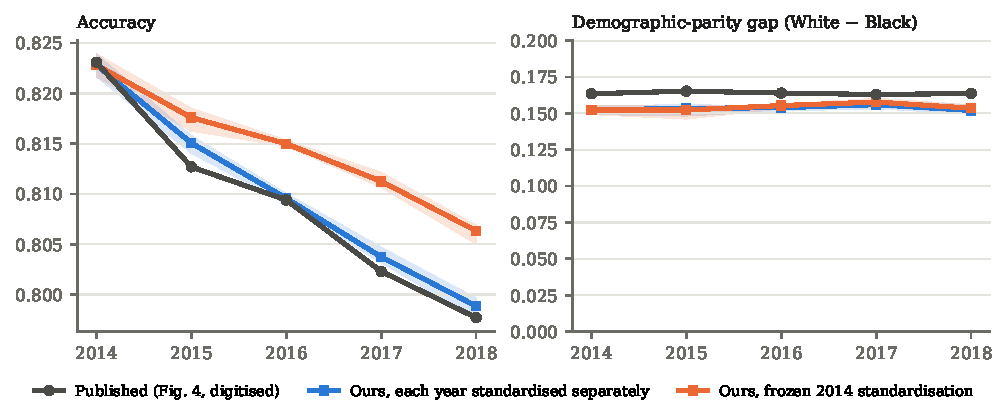
\includegraphics[width=\linewidth]{figures/reconstruction.pdf}
\caption{Reconstruction of \citet[Figure 4]{ding2021retiring}: unconstrained GBM trained on 2014, evaluated on 2014--2018. Published values recovered from the vector figure (grey). Ours: mean over five seeds with min--max band, 100 trees, with each year standardised separately (blue) or with a frozen 2014 standardisation (orange).}
\label{fig:reconstruction}
\end{figure}

% ------------------------------------------------------------------
\section{Pre-registered design}
\label{sec:design}
\todo{condense prereg sections 3--7: data and harmonisation, frozen models, the claim-to-estimand table (C1--C4, C6, C7 confirmatory; C5 secondary; C8 descriptive), calibration constants (values), decision rules and their simulated operating characteristics, weights.}

\section{Results: does the claim hold after 2018?}
\label{sec:results}
\todo{Stage B.}

\section{Why is fairness more stable over time than across states?}
\label{sec:explanation}
\todo{Stage B: C7, C8, decomposition, P1--P3.}

\section{Discussion}
\todo{implications for certificate validity and monitoring; benchmark practice (preprocessing per year, nominal labels, code breaks); limitations.}

\subsubsection*{Reproducibility and pre-registration}
\todo{archive date and SHA-256 of the plan, withheld links during review, deviations.}

\bibliography{main}
\bibliographystyle{tmlr}

\appendix
\section{Harmonisation of ACS codes, 2014--2024}
\label{app:harmonisation}
\todo{tables from results/harmonisation.}

\end{document}
